\documentclass{emulateapj}
\bibliographystyle{astroads}

%define general packages
\usepackage{epsfig}
\usepackage{amsmath}
\usepackage{natbib}
\usepackage{afterpage}
\usepackage{xcolor}
\newcommand\writingnote[1]{\textcolor{red}{#1}}
% \renewcommand\writingnote[1]{}
% \renewcommand\actpol[1]{}
\newcommand{\LCDM}   {$\Lambda$CDM}
\newcommand{\planck}{{\it Planck}}
\newcommand{\wmap}{{\it WMAP}}

\DeclareMathAlphabet\mathbfcal{OMS}{cmsy}{b}{n}
\newcommand{\prr}{ \mathcal{P}_{\mathcal{R}\mathcal{R}} }
\newcommand{\pri}{ \mathcal{P}_{\mathcal{R}\mathcal{I}} }
\newcommand{\pii}{ \mathcal{P}_{\mathcal{I}\mathcal{I}} }


\begin{document}

\title{Future constraints on isocurvature fluctuations from the Cosmic Microwave Background}
\author{Zack Li and Jo Dunkley}
\date{\today}
%\maketitle
\affil{Astrophysical Sciences, Princeton University, Princeton NJ 08544}


\begin{abstract}
We provide forecasts of cold dark matter isocurvature (CDI) constraints for combinations of Planck, CMB S4, and PIXIE. Using MCMC methods on fiducial power spectra, we find substantial improvements in the measurement of the large scale isocurvature power.
\end{abstract}

%Section heading
\section{Introduction}

Current cosmological data support the standard `\LCDM' cosmological model, a flat universe with primordial fluctuations that are scalar, adiabatic, and Gaussian, and are described by a power spectrum with an amplitude and power-law spectral index \citep{planck}. The adiabatic nature of the fluctuations come from a spatially uniform equation of state and initial velocity field and lock together the density perturbations of the different components \citep{planckXXII:2013}. The physical origin of the primordial fluctuations is still not known however, and the most general perturbations include not only adiabatic fluctuations, but also isocurvature perturbations, with spatially varying equations of state or initial velocity fields \citep{adiab}. A non-zero level of isocurvature fluctuations is still allowed by current data.

Isocurvature fluctuations can take the form of variations between the photon and the cold dark matter (CDM) density, the photon and baryon density, or the photon and neutrino density \citep{moodley/bucher/turok:2000}. Variations between the photon velocity and neutrino velocity are also possible. Within an inflation scenario with a single scalar field and slow-roll initial conditions, only adiabatic perturbations are expected. However, isocurvature fluctuations could be generated from a variety of physical scenarios including multiple field inflation \citep{langlois:1999}, and the curvaton scenario
%which generates CDM isocurvature perturbations correlated with the adiabatic modes
\citep{baumann/etal:2009}. Some string theory axions can also generate isocurvature fluctuations from quantum fluctuations, with axion decay to dark matter leading to uncorrelated adiabatic and CDM isocurvature perturbations \cite{axion}. (Mention compensated isocurvature). Early universe models other than inflation could also generate isocurvature.

Data from the \wmap\ satellite, supplemented by Baryon Acoustic Oscillation data, have been used to put upper bounds on the fractional contribution of CDI to the primordial power at less than a percent \citep{hinshaw/etal:2013}, assuming a fixed power-law index and considering either fully uncorrelated or anticorrelated modes. This CDI mode is considered the most physically well-motivated, and is observationally equivalent to baryon isocurvature. Combinations of different isocurvature modes were allowed at a much higher degree \cite{bean}. The \planck\ data reduce the limits on fully correlated power-law CDI to XX, and for a more general partially correlated model limit the fractional power  to be less than 2\% at large scales ($k=0.002$ Mpc$^{-1}$), and less than 52\% at smaller scales ($k=0.1$ Mpc$^{-1}$ \citep{planckXX:2015}.
%These use polarization measurements over the Planck range of $l=2-2508$ for TT and $2-1996$ for TE and EE.

There is still scope for improvement. The isocurvature temperature and polarization power spectra are out of phase with the adiabatic perturbations, so improved CMB polarization measurements can considerably tighten constraints. CMB-S4 is a next-generation ground-based CMB experiment planned for observations in the 2020s, involving hundred of thousands of detectors. It will reduce the polarization noise levels over \planck\ by almost a factor of one hundred, reaching to small angular scales. Proposed low-resolution satellites including PIXIE and LiteBIRD will offer similar improvement for larger angular scales \citep{pixie,litebird}. Forecasts for CMB-S4  predict an increase in sensitivity by a factor of 3-6 over \planck\ for the curvaton scenario \citep{CMB-S4:2016}. \cite{kasanda/moodley:2014} forecast the capabilities of a future CMB satellite, and \cite{smith/grin:2016} forecast that a cosmic-variance limited experiment could reach XX. 
%and investigate the effects of the CMB lensing potential.

In this paper we explore how well the degree of CDI can be constrained with a CMB-S4 level experiment and the proposed PIXIE satellite.  We consider the general CDI model explored by \citet{planck_inflation}, which allows partial correlation of modes and a variable spectral index. 
 %We improve upon these results by including an atmospheric model calibrated for the Atacama desert for CMB-S4, and choose a more general isocurvature model.  While we do not involve PRISM, we do explore combinations of Planck, S4, and PIXIE.
In Section \ref{methods}, we describe the effect of isocurvature on power spectra, our chosen parametrization, and the details of the experimental specifications used in the forecasts. In Section \ref{results}, we present our forecasted constraints, and discuss in section \ref{discussion}.
%we provide some conclusions about the science yield from each experiment and the whether future measurements will be able to differentiate between models for the origin of the primordial density fluctuations.  


\section{Methods}\label{methods}

\begin{figure}[h]
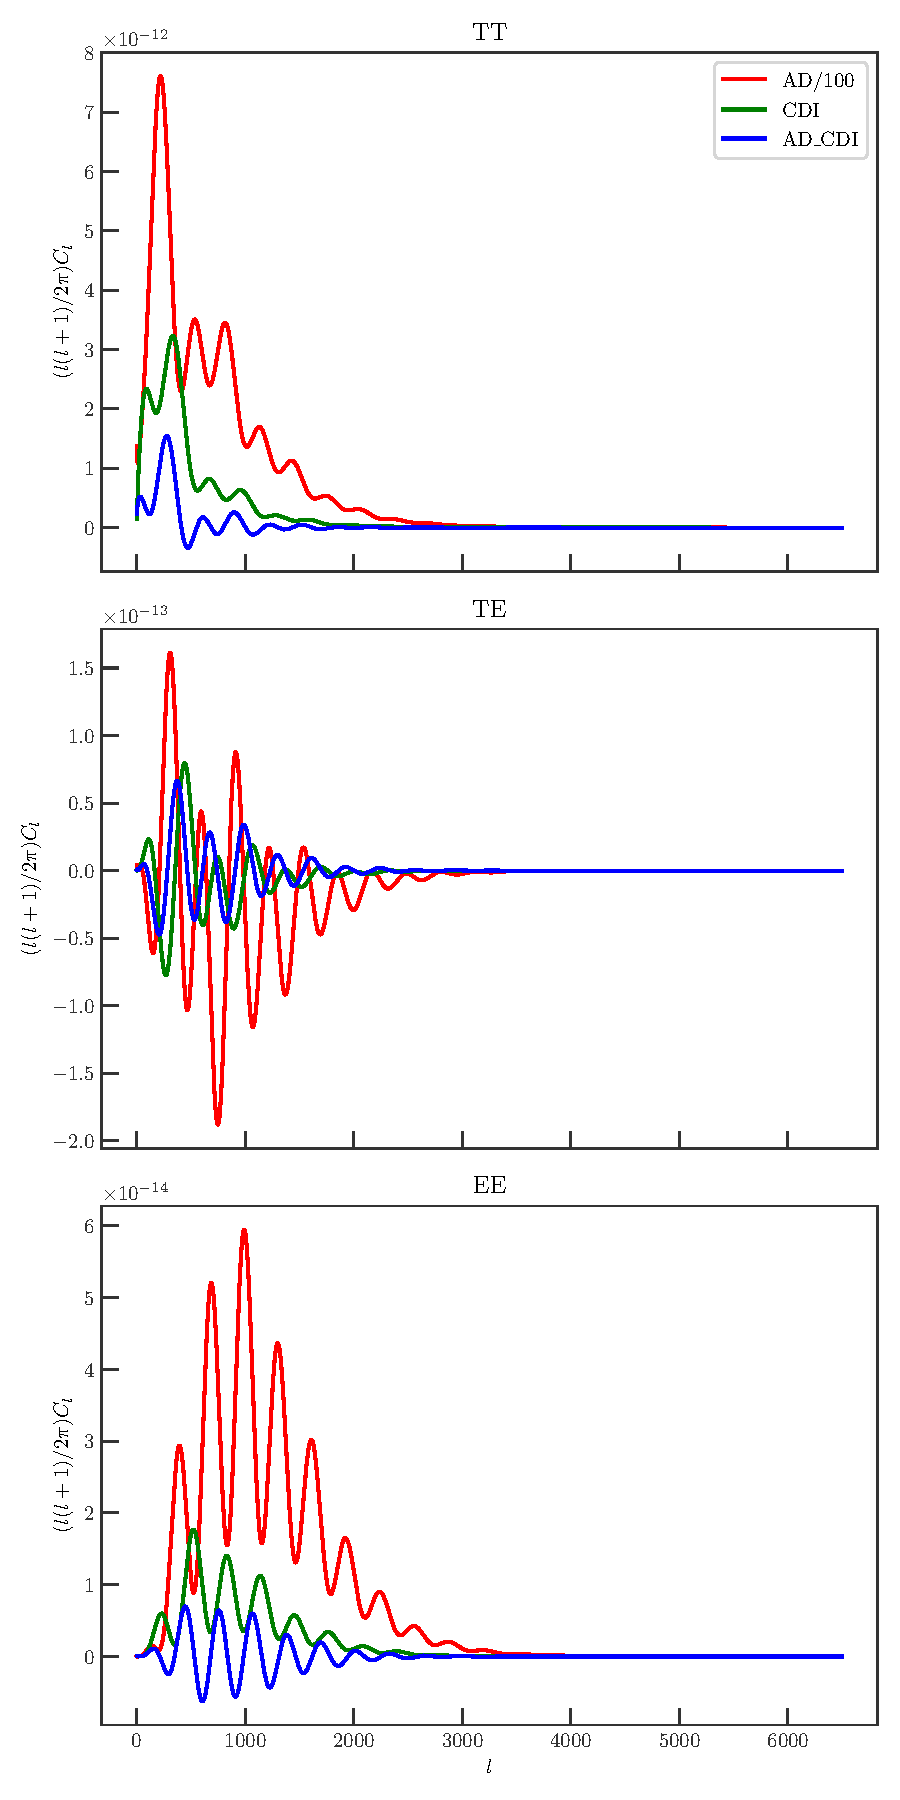
\includegraphics[width=0.45\textwidth]{figures/isocurvature_fiducial_spectra_contributions.pdf}
% \plotone{figures/isocurvature_fiducial_spectra_contributions.pdf}
\caption{Scaled adiabatic and isocurvature contributions to $\mathcal{D}_l$ for a model with nonzero isocurvature consistent with the Planck measurements. \writingnote{overplot ACTPol error bars, plot adiabatic normally and scale isocurvature contributions by 100}\label{fig:effects}}
\end{figure}


\subsection{Perturbations and Power Spectra}\label{powerspectra}

\writingnote{
todo: heuristic description of isocurvature effects on CMB power spectra. maybe I include something like the $dD_l/dP_{II}^j$ plots.
}


Gaussian fluctuations for a general cosmological perturbation are described by a matrix of power spectra, referring to correlations and amplitudes. In this paper, we only consider primordial CDM isocurvature, so the matrix is $2 \times 2$ where $\pii(k)$ is the power spectrum of $\delta \rho_{CDM} / \rho_{CDM}$, with $\rho_{CDM} = n_c / n_{\gamma}$, the ratio of primordial CDM to photon number densities.

\begin{equation}
\mathbfcal{P}(k) = \left( {\begin{array}{cc}
   \prr(k) & \pri(k) \\
   \pri(k) &  \pii(k) \\
  \end{array} } \right)
\end{equation}

Following \cite{planckXX:2015}, we parametrize $\prr$, $\pri$, and $\pii$ by choosing the power at two scales, $k_1 = 0.002$ Mpc$^{-1}$ and $k_2 = 0.100$ Mpc$^{-1}$ and interpolating geometrically,
\begin{align*}
\mathcal{P}_{ab}(k) = & \exp \bigg[ \left( \frac{\ln(k) - \ln(k_2)}{\ln(k_1) - \ln(k_2)}\right) \ln \left( \mathcal{P}_{ab}^1 \right) \\
& +
\left( \frac{\ln(k) - \ln(k_1)}{\ln(k_2) - \ln(k_1)}\right) \ln \left( \mathcal{P}_{ab}^2 \right) \bigg].
\end{align*}
Thus one can recover the tilt by computing the log-log slope,
\begin{equation} n_{\text{ab}}  =  \frac{\log( \mathcal{P}_{\text{ab}}^2 / \mathcal{P}_{\text{ab}}^1 )}{\log ( k_2 / k_1 )}. \end{equation}

For a set of the standard cosmological parameters with the additional isocurvature parameters, we compute a theoretical power spectrum with CLASS, a fast Boltzmann code written in C (citation). The adiabatic and isocurvature are contained in three functions, $\mathcal{P}_{\mathcal{RR}}(k)$, $\mathcal{P}_{\mathcal{II}}(k)$, and $\mathcal{P}_{\mathcal{RI}}(k)$, the curvature, isocurvature, and cross-correlation power spectra, respectively (cite Planck 2015 XX).  We use the same uniform priors as Planck,
\begin{equation}
    \prr^{(1)}, \prr^{(2)} \in (10^{-9}, 10^{-8}),
\end{equation}
\begin{equation}
    \pii^{(1)}, \pii^{(2)} \in (0, 10^{-8}),
\end{equation}
\begin{equation}
    \pri^{(1)} \in (-10^{-8}, 10^{-8}).
\end{equation}
We follow Planck 2015 XX's convention of only sampling over $\pri^1$ and fixing $\pri^{(2)}$ by restricting the correlation fraction to be scale-independent,
\begin{equation}
\cos \Delta_{\text{ab}} = \frac{\mathcal{P}_{\text{ab}}}{(\mathcal{P}_{\text{aa}} \mathcal{P}_{\text{bb}})^{1/2}} \in (-1,1),
\end{equation}
so that
\begin{equation}
\mathcal{P}_{\text{ab}}^{(2)} = \mathcal{P}_{\text{ab}}^{(1)} \frac{\left(\mathcal{P}_{\text{aa}}^{(2)} \mathcal{P}_{\text{bb}}^{(2)} \right)^{1/2}}{ \left(\mathcal{P}_{\text{aa}}^{(1)} \mathcal{P}_{\text{bb}}^{(1)} \right)^{1/2}}.
\end{equation}
We also present the results in terms of derived parameters following \cite{planckXX:2015}, defining the primordial isocurvature fraction as
\begin{equation}
\beta_{\text{iso}}(k) = \frac{\pii(k)}{\prr(k) + \pii(k)}.
\end{equation}

Then we sample over the $\Lambda$CDM scenario, but replace $A_s$ and $n_s$ with $\prr^{(1)}$,  $\prr^{(2)}$ and add the three isocurvature parameters $\pii^{(1)}$, $\pii^{(2)}$, $\pri^{(1)}$.
\begin{align}
\{ \Omega_b h^2, \Omega_c h^2, \theta_A, &\tau_{reio}, \prr^{(1)}, \mathcal{P}_{\mathcal{RR}}^{(2)} \\
& \pii^{(1)}, \pii^{(2)}, \pri^{(1)}    \}
\end{align}

\begin{figure}
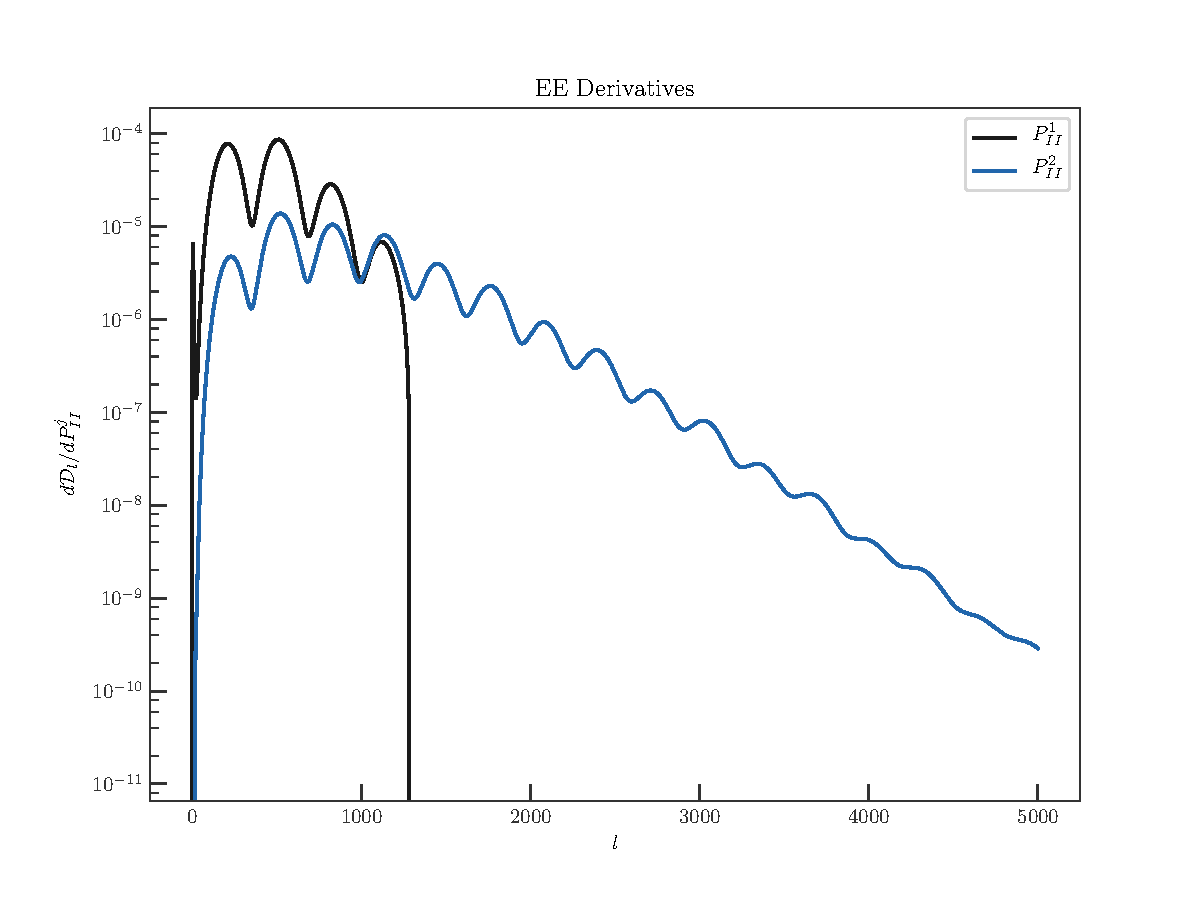
\includegraphics[width=0.5\textwidth]{figures/logee.pdf}
% \plotone{figures/isocurvature_fiducial_spectra_contributions.pdf}
\caption{A measurement of the impact of the two isocurvature powers $\pii^1$ and $\pii^2$, by taking the derivative of $\mathcal{D}_l$ with respect to $\pii^i$, for a model with nonzero isocurvature consistent with the Planck measurements.\label{fig:derivs}}
\end{figure}

\subsection{Forecasting}\label{forecasting}
We create mock likelihoods following \cite{perotto/etal:2006}, in which for each experiment we are using in our forecasts, we estimate an $l$-range, $f_{\text{sky}}$, beam width $\theta_{\text{fwhm}}$, temperature noise $\sigma_T$, and polarization noise $\sigma_P$. Then we have, for $X,Y \in \{T, E, B\}$ \citep{perotto/etal:2006},
\begin{equation}
\mathbf{N}_l^{XY} = \delta_{XY} \theta_{\text{fwhm}}^2 \sigma_X^2 \exp \left[  l(l+1) \frac{\theta_{\text{fwhm}}}{8 \ln 2}  \right]
\end{equation}
The parameters we use for each experiment are in Table \ref{table:forecasts}.

For CMB-S4, we also include a multiplicative factor for atmospheric noise, in the form of a fitting function with $l_{\text{knee}} = 330$, $\alpha = -3.8$,
\begin{equation}
N_l = N_0 \left( 1 + \left(\frac{l}{l_{\text{knee}}}\right)^{\alpha} \right)
\end{equation}

We then use this $N_l$ with a fiducial power spectrum generated in CLASS with the Planck 2015 cosmological parameters \citep{planckXIII:2016}. We investigate both a fiducial spectrum with zero isocurvature, and one a relatively extreme model which is still consistent with the Planck constraints.


\begin{deluxetable*}{cccccc}
\label{table:forecasts}
\tabletypesize{\footnotesize}
\tablecolumns{6}
\tablewidth{0pt}
\tablecaption{ Forecasting Parameters \label{table:forecasts}}
\tablehead{
 \colhead{Experiment}     & \colhead{$l_{min}$ - $l_{max}$}  & \colhead{$f_{\text{sky}}$} & \colhead{$\theta_{\text{FWHM}}$} & \colhead{$\sigma_T$ ($\mu$K arcmin)} &  \colhead{$\sigma_P$ ($\mu$K arcmin)} }
 \startdata
  CMB-S4          & 30-3000 & 0.40 & 3.0 & 1.0 & 1.4\\
  PIXIE           & 2 - 150 & 0.8 & 120 & 2.9 & 4.0 \\
  Planck 2015 high\_l + pol & 2 - 2500 & 0.65 & 10,7.1,5.0 & 65.0, 43.0, 66.0 & 103.0, 81.0, 134.0 \\
\enddata
% \vspace{-0.8cm}
\tablecomments{Noise parameters for CMB-S4 \citep{CMB-S4:2016}, PIXIE (\writingnote{FIND CITATION}), and Planck + Planck Polarization \citep{planckXX:2015}. The three Planck noise levels come from three channels at 70, 100 and 143 GHz respectively.}
\end{deluxetable*}

We find constraints for the isocurvature parameters using these likelihood parameters and Markov Chain Monte Carlo (MCMC) sampling. We use Monte Python, a Python-based implementation of Metropolis-Hastings and interface for cosmological likelihoods. We use six different combinations of experiments.
\begin{enumerate}
\item Planck TT ($2 \leq l \leq 2500$), \\ Planck TEB ($2 \leq l \leq 30$).
\item Planck TEB ($2 \leq l \leq 2500$).
\item Planck TEB ($2 \leq l \leq 30$,) \\CMB-S4 ($30 < l \leq 3000$).
\item PIXIE over ($2 \leq l \leq 150$),\\ Planck TEB ($150 < l  \leq 2500$).
\item PIXIE over ($2 \leq l \leq 150$),\\ CMB-S4 ($150 < l  \leq 2500$).
\end{enumerate}





\section{Results}\label{results}

The bestfit values are $\pii^1 = something$, $\pii^2 = something$.

\writingnote{
  \begin{itemize}
    \item How much does S4 improve the constraint? Numbers! 
    \item What's the effect of low $l$ and high $l$ on these constraints? Refer to figure 1. 
    \item Provide a table with upper bounds on the derived parameters.
    \item PIXIE's improvement on $\prr$ and $\tau$. 
    \item Answer the question "Should I build this experiment to measure isocurvature better?"
    \item Need good polarization, emphasize
    \item $l$ ranges that matter
  \end{itemize}
}

\afterpage{\clearpage}
\begin{figure*}[p]
% \epsscale{.80}
\plotone{figures/forecast_all_overplotted.pdf}
\caption{Isocurvature constraints for future CMB experiments.\label{fig:triangleplots}}
\end{figure*}



\afterpage{\clearpage}
\begin{figure*}[p]
% \epsscale{.80}
\plotone{figures/all_derived_forecast.pdf}
\caption{Derived parameter estimates for future CMB experiments.\label{fig:derivedparams}}
\end{figure*}

\writingnote{
    \begin{itemize}
        \item Write about triangle plot
        \item Write about derived parameters
        \item Make a table summarizing various parameters with errors
    \end{itemize}
}




\subsection{ACTPol Likelihood}\label{actpol}

We also calculated the isocurvature constraints provided by the ACTPol Season 2 polarization data. We use the same methods as in Louis et al. 2016 for the ACT likelihood, marginalizing the ACTPol spectrum from $350 < l < 4000$ to construct a Gaussian likelihood function with an overall calibration parameter. We produce our parameter constraints by summing this with the Planck 2015 likelihood. We use the public CMB-marginalized 'plik-lite' Planck 2015 likelihood which uses TT for $30 \leq l \leq 2508$, a likelihood generated from CMB lensing, and a joint TT, EE, BB, and TE likelihood for the range $2 \leq l < 30$. Introducing ACTPol provided a minor improvement of roughly 10\% in constraining both $\pii^1$ and $\pii^2$.


\section{Discussion}\label{Discussion}
\writingnote{
  \begin{itemize}
    \item can we constrain or rule out theoretical models? 
    \item CMB-S4 -- are there models we can elminate or fit?
    \item fraction of cosmic variance limit?
    \item reiterate that isocurvature is a unique probe of the primordial fluctuations
  \end{itemize}
}

\appendix

\writingnote{comparing the fiducial power spectrum Planck parameter estimates with real Planck}

\bibliography{mybib}

\end{document}
